\subsection{Đề thi thử THPTQG Sở GDĐT HƯNG YÊN 25--26, Lần 2}

\caulc
\Opensolutionfile{ans}[ans/ans-26-2--SoGDHY-L2-LC]
\begin{ex}%[2D4N1-2]
	Khẳng định nào sau đây là đúng?
	\choice
	{$\displaystyle\int(x-3)\mathrm{d}x=2x^{2}-3x+C$}
	{$\displaystyle\int(x-3)\mathrm{d}x=\dfrac{1}{2}x^{2}+3x+C$}
	{\True $\displaystyle\int(x-3)\mathrm{d}x=\dfrac{1}{2}x^{2}-3x+C$}
	{$\displaystyle\int(x-3)\mathrm{d}x=x^{2}-3x+C$}
	\loigiai{
		Ta có $\displaystyle\int(x-3)\mathrm{d}x = \dfrac{x^2}{2} - 3x + C$.
	}
\end{ex}

\begin{ex}%[2D3H1-3]
	Bảng sau đây biểu diễn mẫu số liệu ghép nhóm về cân nặng của một loại cá trước khi thả xuống hồ (đơn vị: kg).
	\begin{center}
		\begin{tabular}{|l|c|c|c|c|c|}
			\hline
			Nhóm & $[1{,}2; 1{,}3)$ & $[1{,}3; 1{,}4)$ & $[1{,}4; 1{,}5)$ & $[1{,}5; 1{,}6)$ & $[1{,}6; 1{,}7)$ \\
			\hline
			Tần số & $14$ & $40$ & $13$ & $10$ & $3$ \\
			\hline
		\end{tabular}
	\end{center}
	Khoảng tứ phân vị của mẫu số liệu ghép nhóm trên (làm tròn đến hàng phần trăm) là
	\choice
	{$0{,}12$}
	{$0{,}14$}
	{$0{,}11$}
	{\True $0{,}13$}
	\loigiai{
		Cỡ mẫu $n = 14 + 40 + 13 + 10 + 3 = 80$.\\
		Vị trí tứ phân vị thứ nhất là $\dfrac{n}{4} = 20$. Do đó $Q_1$ thuộc nhóm $[1{,}3; 1{,}4)$.
		$$Q_1 = 1{,}3 + \dfrac{20-14}{40}\cdot 0{,}1 = 1{,}315.$$
		Vị trí tứ phân vị thứ ba là $\dfrac{3n}{4} = 60$. Do đó $Q_3$ thuộc nhóm $[1{,}4; 1{,}5)$.
		$$Q_3 = 1{,}4 + \dfrac{60-(14+40)}{13}\cdot 0{,}1 =\dfrac{94}{65}$$
		Khoảng tứ phân vị $\Delta_Q = Q_3 - Q_1 =\dfrac{94}{65} - 1{,}315 \approx 0{,}13$.
	}
\end{ex}

\begin{ex}%[2D1H3-1] 
	Giá trị nhỏ nhất của hàm số $f(x)=-2x^{3}+3x^{2}+1$ trên đoạn $[-1;1]$ bằng
	\choice
	{\True $1$}
	{$2$}
	{$0$}
	{$-1$}
	\loigiai{
		Ta có $f'(x) = -6x^2 + 6x$.\\
		Cho $f'(x) = 0 \Leftrightarrow -6x^2 + 6x = 0 \Leftrightarrow \hoac{&x=0 \in [-1;1]\\&x=1 \in [-1;1].}$\\
		Tính các giá trị: $f(-1) = 6$, $f(0) = 1$, $f(1) = 2$.\\
		Vậy $\min\limits_{[-1;1]} f(x) = f(0) = 1$.
	}
\end{ex}

\begin{ex}%[2D1N2-2]
	\immini[thm]{Cho hàm số $y=f(x)$ có bảng biến thiên.
		Điểm cực tiểu của hàm số đã cho là
		\choice
		{\True $x=2$}
		{$x=0$}
		{$x=1$}
		{$x=4$}}{
\begin{tikzpicture}
			\tkzTabInit[lgt=1.2,espcl=1.7]
			{$x$ /0.8, $f'(x)$ /0.8, $f(x)$ /1.5}
			{$-\infty$, $0$, $2$, $+\infty$}
			\tkzTabLine{, +, 0, -, 0, +, }
			\tkzTabVar{-/ $-\infty$, +/ $4$, -/ $0$, +/ $+\infty$}
	\end{tikzpicture}}
	\loigiai{
		Từ bảng biến thiên, ta thấy $f'(x)$ đổi dấu từ âm sang dương khi qua $x=2$.\\
		Vậy điểm cực tiểu của hàm số là $x=2$.
	}
\end{ex}

\begin{ex}%[2H5H3-3]
	Trong không gian $Oxyz$, cho hai điểm $A(1;2;3)$ và $B(-2;1;5)$. Phương trình mặt cầu tâm $A$ bán kính $AB$ là
	\choice
	{$(x+1)^{2}+(y+2)^{2}+(z+3)^{2}=28$}
	{\True $(x-1)^{2}+(y-2)^{2}+(z-3)^{2}=14$}
	{$(x+1)^{2}+(y+2)^{2}+(z+3)^{2}=14$}
	{$(x-1)^{2}+(y-2)^{2}+(z-3)^{2}=28$}
	\loigiai{
		Ta có $\vec{AB} = (-3; -1; 2) \Rightarrow R^2 = AB^2 = 14$.\\
		Phương trình mặt cầu tâm $A(1;2;3)$, bán kính $R=AB$ là $(x-1)^{2}+(y-2)^{2}+(z-3)^{2}=14$.
	}
\end{ex}

\begin{ex}%[1H8N7-4]
	\immini[thm]{Cho hình lăng trụ đều $ABC.A'B'C'$ có tất cả các cạnh bằng $4 \text{ cm}$ (xem hình). Thể tích của khối lăng trụ đã cho bằng
		\choice
		{$8\sqrt{3} \text{ cm}^{3}$}
		{$32\sqrt{3} \text{ cm}^{3}$}
		{$24\sqrt{3} \text{ cm}^{3}$}
		{\True $16\sqrt{3} \text{ cm}^{3}$}}{\begin{tikzpicture}[>=stealth, line join=round, line cap=round, scale=0.6,font=\footnotesize]
			\coordinate (A') at (0,0);
			\coordinate (B') at (2,-1.5);
			\coordinate (C') at (5,0);
			\coordinate (A) at ($(A')+(0,4)$);
			\coordinate (B) at ($(B')+(0,4)$);
			\coordinate (C) at ($(C')+(0,4)$);
			\draw[dashed] (A')--(C');
			\draw (A')--(B')--(C') (A)--(B)--(C)--cycle (A)--(A') (B)--(B') (C)--(C');
			\draw (A) node[above left] {$A$};
			\draw (B) node[right] {$B$};
			\draw (C) node[above right] {$C$};
			\draw (A') node[left] {$A'$};
			\draw (B') node[below] {$B'$};
			\draw (C') node[right] {$C'$};
	\end{tikzpicture}}
	\loigiai{
		Vì lăng trụ đã cho là lăng trụ đều nên chiều cao $h = 4 \text{ cm}$ và đáy là tam giác đều cạnh $a = 4 \text{ cm}$.\\
		Diện tích đáy là $S = \dfrac{a^2\sqrt{3}}{4} = \dfrac{4^2\sqrt{3}}{4} = 4\sqrt{3} \text{ (cm}^2\text{)}$.\\
		Thể tích khối lăng trụ là $V = S \cdot h = 4\sqrt{3} \cdot 4 = 16\sqrt{3} \text{ (cm}^3\text{)}$.
	}
\end{ex}

\begin{ex}%[1D2N2-2]
	Cho cấp số cộng $(u_n)$ có $u_{2}=2$, $u_{3}=6$. Công sai của cấp số cộng đã cho bằng
	\choice
	{$-4$}
	{\True $4$}
	{$-3$}
	{$3$}
	\loigiai{
		Công sai của cấp số cộng là $\mathrm{D} = u_3 - u_2 = 6 - 2 = 4$.
	}
\end{ex}

\begin{ex}%[2D4H3-1]
	Hình phẳng giới hạn bởi đồ thị hàm số $y=-x^{2}+2x$ và trục $Ox$ có diện tích bằng
	\choice
	{$\dfrac{2}{3}$}
	{$\dfrac{8}{3}$}
	{$\dfrac{20}{3}$}
	{\True $\dfrac{4}{3}$}
	\loigiai{
		Phương trình hoành độ giao điểm của đồ thị hàm số và trục $Ox$:
		$-x^2+2x=0 \Leftrightarrow \hoac{&x=0\\&x=2.}$\\
		Diện tích hình phẳng cần tìm là
		$S = \displaystyle\int\limits_0^2 |-x^2+2x| \mathrm{d}x = \displaystyle\int\limits_0^2 (-x^2+2x) \mathrm{d}x = \left(-\dfrac{x^3}{3}+x^2\right)\bigg|_0^2 = \dfrac{4}{3}$.
	}
\end{ex}

\begin{ex}%[1H8N2-5]
	\immini[thm]{Cho hình chóp $S.ABCD$ có đáy $ABCD$ là hình vuông và $SA \perp (ABCD)$ (xem hình).	Đường thẳng nào sau đây là hình chiếu của $SC$ trên mặt phẳng $(SAB)$?
		\choice
		{$BC$}
		{\True $SB$}
		{$SA$}
		{$AB$}}{\begin{tikzpicture}[>=stealth, line join=round, line cap=round, scale=0.8]
			\coordinate (A) at (0,0);
			\coordinate (B) at (-1.5,-1.5);
			\coordinate (D) at (3,0);
			\coordinate (C) at ($(B)+(D)-(A)$);
			\coordinate (S) at (0,3);
			\draw[dashed] (A)--(B) (A)--(D) (S)--(A);
			\draw (S)--(B)--(C)--(D)--cycle (S)--(C);
			\draw (A) node[below right] {$A$};
			\draw (B) node[below left] {$B$};
			\draw (C) node[below right] {$C$};
			\draw (D) node[right] {$D$};
			\draw (S) node[above] {$S$};
	\end{tikzpicture}}
	\loigiai{
		Ta có $BC \perp AB$ (do $ABCD$ là hình vuông) và $BC \perp SA$ (do $SA \perp (ABCD)$).\\
		Suy ra $BC \perp (SAB)$, nên hình chiếu vuông góc của điểm $C$ lên $(SAB)$ là điểm $B$.\\
		Mặt khác, $S \in (SAB)$ nên hình chiếu vuông góc của $S$ lên $(SAB)$ là chính nó.\\
		Vậy đường thẳng $SB$ là hình chiếu vuông góc của đường thẳng $SC$ lên mặt phẳng $(SAB)$.
	}
\end{ex}

\begin{ex}%[2H5N1-2]
	Trong không gian $Oxyz$, cho đường thẳng $d\colon \dfrac{x+1}{-2}=\dfrac{y-2}{1}=\dfrac{z+3}{-2}$. Vectơ nào dưới đây là một vectơ chỉ phương của $d$?
	\choice
	{$\vec{u_{1}}=(1;-2;3)$}
	{\True $\vec{u_{3}}=(2;-1;2)$}
	{$\vec{u_{2}}=(-2;1;2)$}
	{$\vec{u_{4}}=(-1;2;-3)$}
	\loigiai{
		Đường thẳng $d$ có một vectơ chỉ phương là $\vec{u} = (-2; 1; -2)= - (2; -1; 2)$.
	}
\end{ex}

\begin{ex}%[1D6N4-3]
	Tập nghiệm của bất phương trình $\log_{2}(3x) \ge 3$ là
	\choice
	{$[2;+\infty)$}
	{$\left(0;\dfrac{8}{3}\right]$}
	{$\left(-\infty;\dfrac{8}{3}\right]$}
	{\True $\left[\dfrac{8}{3};+\infty \right)$}
	\loigiai{
		Điều kiện xác định: $3x > 0 \Leftrightarrow x > 0$.\\
		Ta có: $\log_{2}(3x) \ge 3 \Leftrightarrow 3x \ge 2^3 \Leftrightarrow 3x \ge 8 \Leftrightarrow x \ge \dfrac{8}{3}$ (thoả mãn điều kiện).\\
		Vậy tập nghiệm của bất phương trình là $\left[\dfrac{8}{3};+\infty\right)$.
	}
\end{ex}

\begin{ex}%[2D6H1-2]
	Cho hai biến cố $A$, $B$ thoả mãn $\mathrm{P}(A)=0{,}6;$ $\mathrm{P}(B)=0{,}3;$ $\mathrm{P}(B \mid A)=0{,}2.$ Khi đó{,} $\mathrm{P}(A \mid B)$ bằng
	\choice
	{$0{,}45$}
	{$0{,}5$}
	{\True $0{,}4$}
	{$0{,}25$}
	\loigiai{
		Áp dụng công thức nhân xác suất, ta có:
		$\mathrm{P}(A \cap B) = \mathrm{P}(A) \cdot \mathrm{P}(B \mid A) = 0{,}6 \cdot 0{,}2 = 0{,}12$.\\
		Khi đó, $\mathrm{P}(A \mid B) = \dfrac{\mathrm{P}(A \cap B)}{\mathrm{P}(B)} = \dfrac{0{,}12}{0{,}3} = 0{,}4$.
	}
\end{ex}

\Closesolutionfile{ans}


\cauds
\Opensolutionfile{ans}[ans/ans-26-2--SoGDHY-L2-DS]
\begin{ex}%[2D1V4-3]
	Cho hàm số $y=\dfrac{x^{2}+3x+3}{x+2}$ có đồ thị là $(C)$.
	\choiceTF
	{\True Tiệm cận xiên của đồ thị $(C)$ là đường thẳng có phương trình $y=x+1$}
	{Hàm số nghịch biến trên khoảng $(-3;-1)$}
	{Khoảng cách hai điểm cực trị của đồ thị $(C)$ bằng $5\sqrt{2}$}
	{Gọi $I$ là giao điểm hai đường tiệm cận của đồ thị $(C)$. Điểm $M$ thay đổi trên $(C)$, giá trị nhỏ nhất của khoảng cách $IM$ bằng $2\sqrt{2}-2$}
	\loigiai{
		\begin{itemchoice}
			\itemch Ta có $y = \dfrac{x^2+3x+3}{x+2} = x + 1 + \dfrac{1}{x+2}$.\\
			Do $\lim\limits_{x \to \pm\infty} \dfrac{1}{x+2} = 0$ nên tiệm cận xiên của đồ thị $(C)$ là đường thẳng $y=x+1$.
			\itemch Tập xác định $\mathrm{D} = \mathbb{R} \setminus \{-2\}$.\\
			Ta có $y' = \dfrac{x^2+4x+3}{(x+2)^2}$. Cho $y'=0 \Leftrightarrow \hoac{&x=-1\\&x=-3.}$\\
			Hàm số nghịch biến trên các khoảng $(-3;-2)$ và $(-2;-1)$.\\
			Bảng biến thiên
			\begin{center}
				
\begin{tikzpicture}
					\tkzTabInit[nocadre=false,lgt=1.2,espcl=2.5,deltacl=0.6]
					{$x$ /0.6,$y'$ /0.6,$y$ /2}
					{$-\infty$,$-3$,$-2$,$-1$,$+\infty$}
					\tkzTabLine{,+,0,-,d,-,0,+,}
					\tkzTabVar{-/$-\infty$,+/$-3$,-D+/$-\infty$/$+\infty$,-/$1$,+/$+\infty$}
				\end{tikzpicture}
			\end{center}
			Hàm số không liên tục tại $x=-2$ nên không thể nghịch biến trên khoảng $(-3;-1)$.
			\itemch Các điểm cực trị của đồ thị hàm số là $A(-3;-3)$ và $B(-1;1)$.\\
			Khoảng cách $AB = \sqrt{(-1 - (-3))^2 + (1 - (-3))^2} = 2\sqrt{5} \neq 5\sqrt{2}$.
			\itemch Đường tiệm cận đứng là $x = -2$, tiệm cận xiên là $y = x+1$.\\
			Giao điểm hai đường tiệm cận là $I(-2;-1)$.\\
			Điểm $M \in (C)$ nên $M\left(m; m+1+\dfrac{1}{m+2}\right)$ (với $m \neq -2$).\\
			$IM^2 = (m+2 - (-2))^2 + \left(m+1+\dfrac{1}{m+2} - (-1)\right)^2 = 2(m+2)^2 + \dfrac{1}{(m+2)^2} + 2$.\\
			Áp dụng bất đẳng thức AM-GM: $2(m+2)^2 + \dfrac{1}{(m+2)^2} \ge 2\sqrt{2}$.\\
			Dấu \lq\lq$=$\rq\rq, xảy ra khi $(m+2)^4 = \dfrac{1}{2} \Leftrightarrow (m+2)^2 = \dfrac{1}{\sqrt{2}}$.\\
			Suy ra $IM^2 \ge 2\sqrt{2} + 2 \Rightarrow IM \ge \sqrt{2\sqrt{2}+2}$.\\
			Vậy giá trị nhỏ nhất của $IM$ không phải là $2\sqrt{2}-2$.
		\end{itemchoice}
	}
\end{ex}

\begin{ex}%[2H5V3-4]
	Trong không gian $Oxyz$, cho ba điểm $A(2;1;-1)$, $B(3;0;1)$, $C(2;-1;3)$ và mặt cầu $(S)\colon x^{2}+y^{2}+z^{2}-4x+2y-4z+5=0$.
	\choiceTF
	{Mặt phẳng $(ABC)$ tiếp xúc với mặt cầu $(S)$}
	{\True Độ dài đoạn thẳng $AB$ bằng $\sqrt{6}$}
	{Phương trình mặt phẳng $(ABC)$ là $x+y+z-2=0$}
	{\True Điểm $M(x;y;z)$ di động trên mặt cầu $(S)$. Giá trị lớn nhất của biểu thức $P=MA^{2}+2MB^{2}-MC^{2}$ bằng $26+8\sqrt{14}$}
	\loigiai{
		\begin{itemchoice}
			\itemch Mặt cầu $(S)$ có tâm $I(2;-1;2)$ và bán kính $R = \sqrt{2^2+(-1)^2+2^2-5} = 2$.\\
			Ta có $\vec{AB} = (1;-1;2)$, $\vec{AC} = (0;-2;4) \Rightarrow [\vec{AB},\vec{AC}] = (0;-4;-2)$.\\
			Mặt phẳng $(ABC)$ đi qua $A(2;1;-1)$ và có một VTPT $\vec{n} = (0;2;1)$ nên\\
			$(ABC)$ là: $2(y-1) + 1(z+1) = 0 \Leftrightarrow 2y+z-1=0$.\\
			Khoảng cách từ $I$ đến $(ABC)$ là $d(I, (ABC)) = \dfrac{|2(-1)+2-1|}{\sqrt{0^2+2^2+1^2}} = \dfrac{1}{\sqrt{5}} \neq R=2$.\\
			Do đó mặt phẳng $(ABC)$ không tiếp xúc với $(S)$.
			\itemch Ta có $AB = \sqrt{(3-2)^2 + (0-1)^2 + (1 - (-1))^2} = \sqrt{6}$.
			\itemch Mặt phẳng $(ABC)$ có phương trình là $2y+z-1=0$.
			\itemch Gọi $K$ là điểm thoả mãn $\vec{KA} + 2\vec{KB} - \vec{KC} = \vec{0} \Rightarrow \vec{OK} = \dfrac{\vec{OA} + 2\vec{OB} - \vec{OC}}{1 + 2 - 1} = (3;1;-1)$. Điểm $K(3;1;-1)$.
			Khi đó \begin{align*}
				P &= MA^2 + 2MB^2 - MC^2 \\
				&= \left( \vec{MK} + \vec{KA} \right)^2 + 2\left( \vec{MK} + \vec{KB} \right)^2 - \left( \vec{MK} + \vec{KC} \right)^2 \\
				&= 2MK^2 + KA^2 + 2KB^2 - KC^2 \\
				&= 2MK^2 + 1^2 + 2 \cdot \left(\sqrt{5}\right)^2 - \left(\sqrt{21}\right)^2 \\
				&= 2MK^2 - 10.
			\end{align*}
			$P$ đạt giá trị lớn nhất khi $MK$ lớn nhất.\\
			Vì $M \in (S)$ nên $MK \le IK + R = \sqrt{(3-2)^2 + (1 - (-1))^2 + (-1-2)^2} + 2 = \sqrt{14} + 2$.\\
			Vậy $P_{\max} = 2(\sqrt{14}+2)^2 - 10 = 26 + 8\sqrt{14}$.
		\end{itemchoice}
	}
\end{ex}

\begin{ex}%[2D6V2-4]
	Có hai phác đồ điều trị A và B cho một loại bệnh. Phác đồ A có xác suất chữa khỏi bệnh là $55\%$ và xác suất gây tác dụng phụ nghiêm trọng là $8\%$. Phác đồ B có xác suất chữa khỏi bệnh là $75\%$ và xác suất gây tác dụng phụ nghiêm trọng là $12\%$. Một bệnh nhân được điều trị ngẫu nhiên bằng một trong hai phác đồ (xác suất chọn mỗi phác đồ là $50\%$).
	\choiceTF
	{Biết rằng bệnh nhân này gặp tác dụng phụ nghiêm trọng, xác suất bệnh nhân đã được điều trị bằng phác đồ B lớn hơn $0{,}60$}
	{Xác suất bệnh nhân điều trị bằng phác đồ A và được chữa khỏi bệnh là $0{,}55$}
	{\True Xác suất để bệnh nhân bị tác dụng phụ nghiêm trọng là $0{,}10$}
	{Biết rằng trong mỗi phác đồ điều trị thì biến cố \lq \lq bệnh nhân được chữa khỏi bệnh\rq \rq và biến cố \lq \lq bệnh nhân không bị tác dụng phụ nghiêm trọng\rq \rq là độc lập với nhau. Xác suất bệnh nhân khỏi bệnh và không bị tác dụng phụ nghiêm trọng là $0{,}615$}
	\loigiai{
		\begin{itemchoice}
			\itemch Gọi $A, B$ lần lượt là biến cố bệnh nhân điều trị theo phác đồ A, B.\\
			Khi đó $\mathrm{P}(A) = \mathrm{P}(B) = 0{,}5$.\\
			Gọi $T$ là biến cố bệnh nhân gặp tác dụng phụ nghiêm trọng.\\
			Ta có $\mathrm{P}(T) = \mathrm{P}(A)\mathrm{P}(T \mid A) + \mathrm{P}(B)\mathrm{P}(T \mid B) = 0{,}5 \cdot 0{,}08 + 0{,}5 \cdot 0{,}12 = 0{,}10$.\\
			Xác suất bệnh nhân được điều trị bằng phác đồ B biết rằng bệnh nhân gặp tác dụng phụ là $\mathrm{P}(B \mid T) = \dfrac{\mathrm{P}(B \cap T)}{\mathrm{P}(T)} = \dfrac{0{,}5 \cdot 0{,}12}{0{,}10} = 0{,}60$. (Bằng $0{,}60$, không lớn hơn).
			\itemch Gọi $K$ là biến cố bệnh nhân khỏi bệnh.\\
			Xác suất bệnh nhân điều trị bằng phác đồ A và được chữa khỏi là\\
			$\mathrm{P}(A \cap K) = \mathrm{P}(A)\mathrm{P}(K \mid A) = 0{,}5 \cdot 0{,}55 = 0{,}275$.
			\itemch Xác suất để bệnh nhân bị tác dụng phụ nghiêm trọng là $\mathrm{P}(T) = 0{,}10$.
			\itemch Xác suất khỏi bệnh và không bị tác dụng phụ khi dùng phác đồ A:\\ $P_A = \mathrm{P}(K \mid A) \cdot \mathrm{P}(\overline{T} \mid A) = 0{,}55 \cdot (1 - 0{,}08) = 0{,}506$.\\
			Xác suất khỏi bệnh và không bị tác dụng phụ khi dùng phác đồ B:\\ $P_B = \mathrm{P}(K \mid B) \cdot \mathrm{P}(\overline{T} \mid B) = 0{,}75 \cdot (1 - 0{,}12) = 0{,}66$.\\
			Xác suất bệnh nhân khỏi bệnh và không bị tác dụng phụ là:\\ $0{,}5 \cdot 0{,}506 + 0{,}5 \cdot 0{,}66 = 0{,}583 \neq 0{,}615$.
		\end{itemchoice}
	}
\end{ex}

\begin{ex}%[2D4V2-6] 
	Một người điều khiển ô tô đang ở đường dẫn muốn nhập làn vào đường cao tốc. Khi ô tô cách điểm nhập làn $210 \text{ m}$, tốc độ của ô tô là $36 \text{ km/h}$. Ba giây sau đó, ô tô bắt đầu tăng tốc với tốc độ $v(t)=at+b$ $(a,b\in\mathbb{R},a>0)$, trong đó $t$ là thời gian tính bằng giây kể từ khi bắt đầu tăng tốc. Biết rằng ô tô nhập làn cao tốc sau $12$ giây và duy trì sự tăng tốc trong $24$ giây kể từ khi bắt đầu tăng tốc.
	\begin{center}
		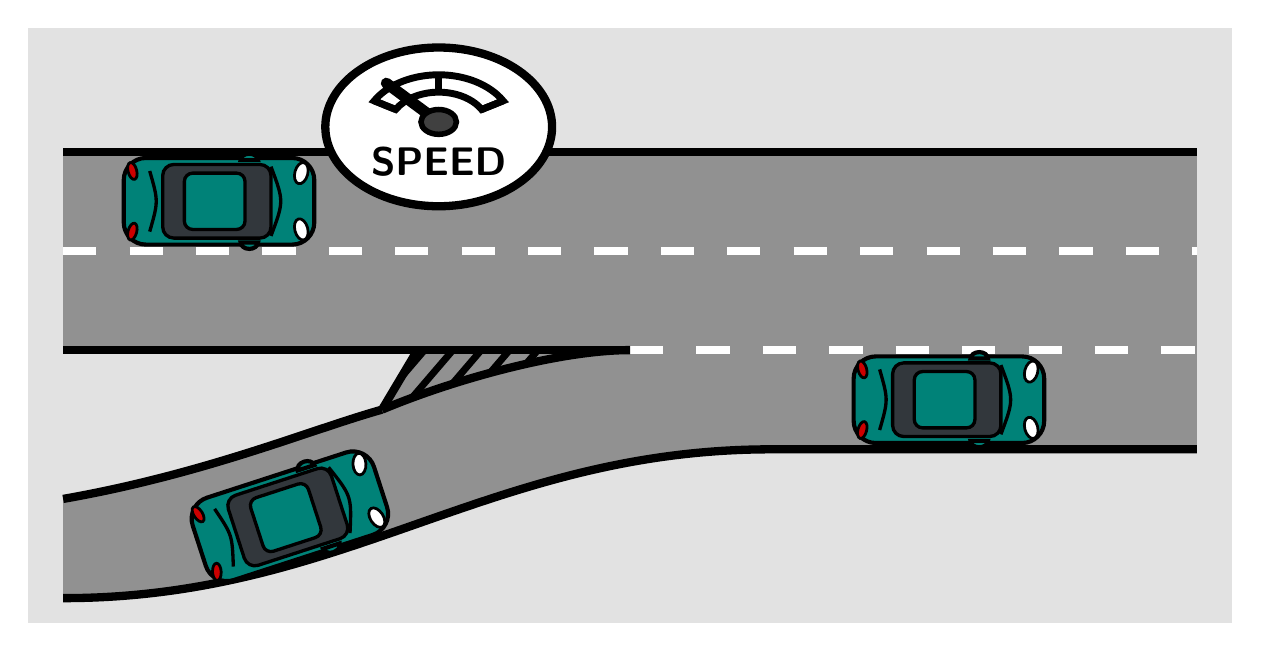
\begin{tikzpicture}[scale=0.9, >=stealth,font=\footnotesize,yscale=0.7]
			
			% ==========================================
			% 1. ĐỊNH NGHĨA MÀU SẮC
			% ==========================================
			\definecolor{bgcol}{RGB}{226, 226, 226}    % Màu nền xám nhạt
			\definecolor{roadcol}{RGB}{145, 145, 145}  % Màu xám mặt đường
			\definecolor{carcol}{RGB}{0, 130, 120}     % Màu xanh ngọc của xe
			\definecolor{glasscol}{RGB}{50, 55, 60}    % Màu xám đậm của kính xe
			
			% ==========================================
			% 2. ĐỊNH NGHĨA ĐỐI TƯỢNG (PIC): XE Ô TÔ
			% ==========================================
			\tikzset{
				car/.pic={
					\begin{scope}[scale=0.55]
						% Thân xe chính
						\draw[line width=1.5pt, fill=carcol, rounded corners=8pt] (-2.2,-1.0) rectangle (2.2,1.0);
						
						% Kính xe (Vẽ một mảng nền kính lớn)
						\draw[line width=1.2pt, fill=glasscol, rounded corners=4pt] (-1.3,-0.85) rectangle (1.2,0.85);
						
						% Nóc xe (Vẽ đè lên mảng kính để tạo kính lái và kính hậu)
						\draw[line width=1.2pt, fill=carcol, rounded corners=3pt] (-0.8,-0.65) rectangle (0.6,0.65);
						
						% Đèn pha (trước)
						\draw[line width=1pt, fill=white, rotate around={-15:(1.9, 0.65)}] (1.9, 0.65) ellipse (0.15 and 0.25);
						\draw[line width=1pt, fill=white, rotate around={15:(1.9,-0.65)}] (1.9,-0.65) ellipse (0.15 and 0.25);
						
						% Đèn hậu (sau)
						\draw[line width=1pt, fill=red!80!black, rotate around={15:(-2.0, 0.7)}] (-2.0, 0.7) ellipse (0.1 and 0.2);
						\draw[line width=1pt, fill=red!80!black, rotate around={-15:(-2.0,-0.7)}] (-2.0,-0.7) ellipse (0.1 and 0.2);
						
						% Gương chiếu hậu
						\draw[line width=1.5pt, fill=carcol] (0.5, 0.95) arc (180:0:0.2 and 0.15) -- cycle;
						\draw[line width=1.5pt, fill=carcol] (0.5,-0.95) arc (-180:0:0.2 and 0.15) -- cycle;
						
						% Đường gân mui xe & cốp xe
						\draw[line width=1.2pt] (1.2, 0.8) .. controls (1.5, 0) .. (1.2, -0.8);
						\draw[line width=1.2pt] (-1.6, 0.7) .. controls (-1.4, 0) .. (-1.6, -0.7);
					\end{scope}
				}
			}
			
			% ==========================================
			% 3. VẼ NỀN (BACKGROUND)
			% ==========================================
			\fill[bgcol] (-0.5, -3.5) rectangle (16.5, 8.5);
			
			% ==========================================
			% 4. VẼ MẶT ĐƯỜNG (LỚP FILL)
			% ==========================================
			\fill[roadcol]
			(0,6) -- (16,6) -- (16,0) -- (10,0)
			.. controls (6,0) and (4,-3.0) .. (0,-3)
			-- (0,-1)
			.. controls (2,-0.5) and (3.5,0.4) .. (4.5,0.8)
			-- (5,2) -- (0,2) -- cycle;
			
			% ==========================================
			% 5. VẼ CÁC VẠCH KẺ ĐƯỜNG
			% ==========================================
			% Vạch đứt nét chia làn 1 và 2 (kéo dài toàn bộ)
			\draw[line width=3pt, white, dashed, dash pattern=on 12pt off 12pt] (0,4) -- (16,4);
			
			% Vạch đứt nét chia làn 2 và 3 (sau khi gộp làn)
			\draw[line width=3pt, white, dashed, dash pattern=on 12pt off 12pt] (8,2) -- (16,2);
			
			% ==========================================
			% 6. VẼ VẠCH XƯƠNG CÁ (HATCHED AREA)
			% ==========================================
			\begin{scope}
				% Tạo giới hạn vùng xương cá
				\clip (5,2) -- (8,2) .. controls (7,2) and (5.5,1.4) .. (4.5,0.8) -- cycle;
				% Vẽ các vạch chéo
				\foreach \i in {0,...,10} {
					\draw[line width=2.5pt] (3.8 + \i*0.4, 0.5) -- (5.0 + \i*0.4, 2.5);
				}
			\end{scope}
			
			% ==========================================
			% 7. VẼ CÁC ĐƯỜNG VIỀN MẶT ĐƯỜNG CHÍNH (SOLID BLACK LINES)
			% ==========================================
			% Viền trên cùng
			\draw[line width=3pt] (0,6) -- (16,6);
			
			% Viền dưới đường chính (bên trái, trước chỗ nối)
			\draw[line width=3pt] (0,2) -- (5,2);
			
			% Viền dưới cùng của nhánh và đường chính bên phải
			\draw[line width=3pt] (16,0) -- (10,0) .. controls (6,0) and (4,-3.0) .. (0,-3);
			
			% Viền trên của nhánh nối (đường cong dưới vùng xương cá)
			\draw[line width=3pt] (0,-1) .. controls (2,-0.5) and (3.5,0.4) .. (4.5,0.8);
			
			% Các cạnh giới hạn vùng xương cá
			\draw[line width=3pt] (5,2) -- (8,2);       % Cạnh trên
			\draw[line width=3pt] (5,2) -- (4.5,0.8);     % Cạnh vát trái
			\draw[line width=3pt] (4.5,0.8) .. controls (5.5,1.4) and (7,2) .. (8,2); % Cạnh cong dưới
			
			% ==========================================
			% 8. CHÈN CÁC XE Ô TÔ VÀO ĐƯỜNG
			% ==========================================
			% Xe 1 (Làn 1, bên trái)
			\pic at (2.2, 5) {car};
			
			% Xe 2 (Làn 3, bên phải)
			\pic at (12.5, 1) {car};
			
			% Xe 3 (Đang đi từ nhánh nối lên, có góc nghiêng)
			\pic at (3.2, -1.35) [rotate=18] {car};
			
			% ==========================================
			% 9. VẼ BIỂU TƯỢNG "SPEED"
			% ==========================================
			\begin{scope}[shift={(5.3, 6.5)}, scale=1]
				% Khung viền biểu tượng
				\draw[line width=3pt, fill=white] (0,0) circle (1.6);
				
				% Vạch cong của đồng hồ đo tốc độ
				\draw[line width=2.5pt] (150:1.05) arc (150:30:1.05) -- (30:0.7) arc (30:150:0.7) -- cycle;
				
				% Các vạch chia nhỏ trên đồng hồ
				\draw[line width=2.5pt] (150:0.7) -- (150:1.05);
				\draw[line width=2.5pt] (90:0.7) -- (90:1.05);
				\draw[line width=2.5pt] (30:0.7) -- (30:1.05);
				
				% Kim đồng hồ chỉ tốc độ
				\draw[line width=4pt, line cap=round] (0,0.1) -- (130:1.15);
				
				% Trục kim đồng hồ (nút tròn giữa)
				\draw[line width=2pt, fill=darkgray] (0,0.1) circle (0.25);
				
				% Chữ "SPEED"
				\node[font=\sffamily\bfseries\Large] at (0, -0.7) {SPEED};
			\end{scope}
			
		\end{tikzpicture}
	\end{center}	
	\choiceTF
	{\True Giá trị của $b$ là $10$}
	{\True Quãng đường ô tô đi được từ khi bắt đầu tăng tốc đến khi nhập làn là $180 \text{ m}$}
	{Sau $24$ giây kể từ khi tăng tốc, tốc độ của ô tô không vượt quá tốc độ tối đa cho phép là $100 \text{ km/h}$}
	{Quãng đường $S(t)$ (đơn vị: mét) mà ô tô đi được trong thời gian $t$ giây $(0\le t\le24)$ kể từ khi tăng tốc được tính theo công thức: $S(t)=\displaystyle\int\limits_{0}^{24}v(t)\mathrm{d}t$}
	\loigiai{
		\begin{itemchoice}
			\itemch Đổi $36 \text{ km/h} = 10 \text{ m/s}$.\\
			Lúc $t=0$, ô tô bắt đầu tăng tốc sau khi đã chạy ổn định $3$ giây với vận tốc $10 \text{ m/s}$.\\
			Vận tốc tại thời điểm bắt đầu tăng tốc là $v(0) = a \cdot 0 + b = b \Rightarrow b = 10$.
			\itemch Trong $3$ giây đầu (trước khi tăng tốc), ô tô đi được quãng đường là $10 \cdot 3 = 30 \text{ m}$.\\
			Vì khoảng cách ban đầu đến điểm nhập làn là $210 \text{ m}$, nên quãng đường ô tô đi được từ khi bắt đầu tăng tốc đến khi nhập làn là $210 - 30 = 180 \text{ m}$.
			\itemch Ô tô nhập làn sau $12$ giây kể từ khi tăng tốc, nên quãng đường đi được là\\ $\displaystyle\int\limits_{0}^{12} (at+10)\mathrm{d}t = 180$ $\Leftrightarrow \left(a\dfrac{t^2}{2} + 10t\right)\bigg|_0^{12} = 180 \Leftrightarrow 72a + 120 = 180 \Leftrightarrow a = \dfrac{5}{6}$.\\
			Phương trình vận tốc là $v(t) = \dfrac{5}{6}t + 10$.\\
			Sau $24$ giây, tốc độ của ô tô là $v(24) = \dfrac{5}{6} \cdot 24 + 10 = 30 \text{ m/s} = 108 \text{ km/h}$.\\
			Tốc độ này lớn hơn $100 \text{ km/h}$.
			\itemch Quãng đường $S(t)$ đi được trong thời gian $t$ giây kể từ khi tăng tốc phải được tính bằng biểu thức tích phân $\displaystyle\int\limits_{0}^{t}v(x)\mathrm{d}x$, trong khi công thức đề bài cho là $\displaystyle\int\limits_0^{24}v(t)\mathrm{d}t$ (đây là một hằng số thể hiện tổng quãng đường đi được trong $24$ giây).
		\end{itemchoice}
	}
\end{ex}
\Closesolutionfile{ans}

\caukq
\Opensolutionfile{ans}[ans/ans-26-2--SoGDHY-L2-KQ]
\begin{ex}%[1D6C4-6]
	\immini[thm]{Gọi $A$ và $B$ là hai điểm phân biệt trên đồ thị của hàm số $y=\log_{3}(5x-3)$ sao cho $A$ là trung điểm của đoạn $OB$. Độ dài đoạn thẳng $AB$ có dạng $\dfrac{\sqrt{a}}{b}$. Tính giá trị $ab$.}{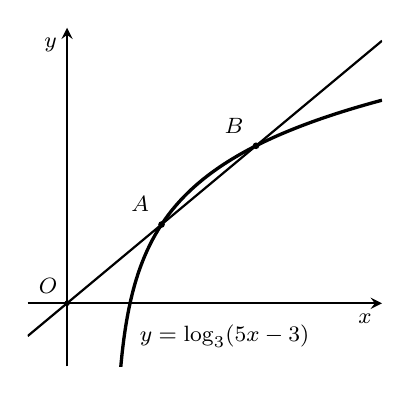
\begin{tikzpicture}[>=stealth, scale=1,font=\footnotesize]
			
			% 1. Khai báo giới hạn trục tọa độ
			\def\xmin{-0.5} 
			\def\xmax{4}
			\def\ymin{-0.8} 
			\def\ymax{3.5}
			
			% 2. Giới hạn vùng vẽ (BẮT BUỘC theo chuẩn)
			\clip (\xmin, \ymin) rectangle (\xmax, \ymax);
			
			% 3. Vẽ hệ trục tọa độ
			\draw[->, thick] (\xmin,0) -- (\xmax,0) node[below left] {$x$};
			\draw[->, thick] (0,\ymin) -- (0,\ymax) node[below left] {$y$};
			\node[above left] at (0,0) { $O$};
			\fill (0,0) circle (1pt);
			
			% 4. Vẽ đồ thị hàm số y = log_3(5x-3)
			% Tiệm cận đứng x = 0.6, ta cho chạy từ x = 0.61 để tránh lỗi tiệm cận
			\draw[very thick, samples=150, domain=0.605:\xmax, smooth] 
			plot (\x, {ln(5*\x-3)/ln(3)});
			
			% Nhãn của đồ thị hàm số
			\node[below] at (2, -0.15) {$y = \log_3(5x - 3)$};
			
			% 5. Vẽ đường thẳng y = 5/6*x đi qua O, A, B
			\draw[thick, domain=\xmin:\xmax, smooth] 
			plot (\x, {5/6*\x});
			
			% 6. Tọa độ chính xác của A và B
			\coordinate (A) at (1.2, 1);
			\coordinate (B) at (2.4, 2);
			
			% Vẽ điểm A
			\fill (A) circle (1.2pt);
			\node[above left=1pt] at (A) {$A$};
			
			% Vẽ điểm B
			\fill (B) circle (1.2pt);
			\node[above left=1pt] at (B) {$B$};
			
	\end{tikzpicture}}
	\shortans[]{305}
	\loigiai{
		Gọi $A(x_1; y_1)$ và $B(x_2; y_2)$ thuộc đồ thị hàm số $y=\log_{3}(5x-3)$. Ta có điều kiện $x > \dfrac{3}{5}$.\\
		Vì $A$ là trung điểm của $OB$ ($O$ là gốc toạ độ) nên $x_2 = 2x_1$ và $y_2 = 2y_1$.\\
		Thay toạ độ $A, B$ vào phương trình hàm số, ta có:
		$\begin{cases}y_1 = \log_3(5x_1 - 3)\\y_2 = \log_3(5x_2 - 3)\end{cases}\\ \Rightarrow 2\log_3(5x_1-3) = \log_3(10x_1-3)$
		$\Leftrightarrow (5x_1-3)^2 = 10x_1-3 \\
		\Leftrightarrow 25x_1^2 - 30x_1 + 9 = 10x_1 - 3$
		$\Leftrightarrow 25x_1^2 - 40x_1 + 12 = 0 \Leftrightarrow \hoac{&x_1 = \dfrac{6}{5}\text{ (thoả mãn)}\\&x_1 = \dfrac{2}{5}\text{ (loại).}}$\\
		Với $x_1 = \dfrac{6}{5} \Rightarrow y_1 = \log_3\left(5\cdot \dfrac{6}{5} - 3\right) = 1$. Suy ra $A\left(\dfrac{6}{5}; 1\right)$.\\
		Vì $A$ là trung điểm của $OB$ nên $AB = OA = \sqrt{\left(\dfrac{6}{5}\right)^2 + 1^2} = \sqrt{\dfrac{61}{25}} = \dfrac{\sqrt{61}}{5}$.\\
		Từ đó suy ra $a = 61$, $b = 5$. Vậy $ab = 61 \cdot 5 = 305$.
	}
\end{ex}

\begin{ex}%[2H5C2-8] 
	Trong không gian $Oxyz$, cho điểm $C(0;6;1)$ và đường thẳng $\Delta$ song song với trục $Oz$. Một điểm $M$ di động trên $\Delta$ sao cho $0\le z_M\le 10$. Biết rằng tổng khoảng cách từ hai điểm $A(3;0;0)$ và $B(-3;0;0)$ đến $\Delta$ bằng $2\sqrt{34}$. Khi khoảng cách $MC$ ngắn nhất, điểm $M$ trùng với $M_{0}(x_{0};y_{0};z_{0})$. Tính $S=x_{0}+20y_{0}+11z_{0}$.
	\shortans[]{111}
	\loigiai{
		Đường thẳng $\Delta$ song song với $Oz$ nên cắt mặt phẳng $(Oxy)$ tại một điểm $H(x_0; y_0; 0)$.\\
		Khi đó phương trình $\Delta$ có dạng $\begin{cases} x = x_0 \\ y = y_0 \\ z = t. \end{cases}$\\
		Khoảng cách từ $A(3;0;0)$ và $B(-3;0;0)$ đến $\Delta$ lần lượt là $HA$ và $HB$.\\
		Theo giả thiết: $HA + HB = 2\sqrt{34} \Leftrightarrow \sqrt{(x_0-3)^2 + y_0^2} + \sqrt{(x_0+3)^2 + y_0^2} = 2\sqrt{34}$.\\
		Tập hợp điểm $H(x_0;y_0)$ trong mặt phẳng $(Oxy)$ là một elip có tiêu điểm $A, B$ với
		Trục lớn $2a = 2\sqrt{34} \Rightarrow a = \sqrt{34}$.\\
		Tiêu cự $2c = AB = 6 \Rightarrow c = 3$.\\
		Trục bé $b = \sqrt{a^2-c^2} = \sqrt{34-9} = 5$.\\
		Phương trình elip là $(E)\colon \dfrac{x_0^2}{34} + \dfrac{y_0^2}{25} = 1 \Rightarrow x_0^2 = 34 - \dfrac{34}{25}y_0^2$ (với $y_0 \in [-5; 5]$).\\
		Khoảng cách $MC^2 = (x_M - 0)^2 + (y_M - 6)^2 + (z_M - 1)^2 = x_0^2 + (y_0 - 6)^2 + (z_M - 1)^2$.\\
		Để $MC$ ngắn nhất thì $(z_M - 1)^2$ phải nhỏ nhất và $x_0^2 + (y_0 - 6)^2$ phải nhỏ nhất.\\
		Do $0 \le z_M \le 10$ nên $(z_M - 1)^2 \ge 0$, đạt min khi $z_M = z_0 = 1$.\\
		Xét $f(y_0) = x_0^2 + (y_0 - 6)^2 = 34 - \dfrac{34}{25}y_0^2 + y_0^2 - 12y_0 + 36 = 70 - \dfrac{9}{25}y_0^2 - 12y_0$ với $y_0 \in [-5;5]$.\\
		Ta có $f'(y_0) = -\dfrac{18}{25}y_0 - 12 < 0, \forall y_0 \in [-5;5]$.\\
		Do đó hàm số nghịch biến trên $[-5;5]$, suy ra $\min f(y_0) = f(5) = 70 - 9 - 60 = 1$.\\
		Khi $y_0 = 5$, ta có $x_0^2 = 34 - \dfrac{34}{25}\cdot 25 = 0 \Rightarrow x_0 = 0$.\\
		Vậy điểm $M_0(0; 5; 1)$, tức là $x_0 = 0$, $y_0 = 5$, $z_0 = 1$.\\
		$S = 0 + 20(5) + 11(1) = 111$.
	}
\end{ex}

\begin{ex}%[2D1V5-8] 
	Một xưởng sản xuất robot hút bụi thông minh đang trong giai đoạn tăng tốc. Số lượng robot sản xuất mỗi tháng là $x$ (chiếc), với $x\in\mathbb{N}^{*}$ và $10\le x\le500$. Mỗi robot được bán với giá cố định là $12$ triệu đồng, tổng chi phí sản xuất mỗi tháng là $C(x)=150\cdot \mathrm{e}^{0{,}005x}+450$ (triệu đồng). Để xưởng đạt lợi nhuận tối thiểu là $1{,}5$ tỷ đồng mỗi tháng, xưởng cần sản xuất và tiêu thụ ít nhất bao nhiêu robot một tháng?
	\shortans[]{196}
	\loigiai{
		Đổi $1{,}5 \text{ tỷ đồng} = 1500 \text{ triệu đồng}$.\\
		Hàm lợi nhuận mỗi tháng là: $\mathrm{P}(x) = 12x - C(x) = 12x - 150\cdot \mathrm{e}^{0{,}005x} - 450$.\\
		Theo yêu cầu bài toán, ta cần tìm $x \in \mathbb{N}^*$ nhỏ nhất thoả mãn $\mathrm{P}(x) \ge 1500$.\\
		$\Leftrightarrow 12x - 150\cdot \mathrm{e}^{0{,}005x} - 450 \ge 1500 \Leftrightarrow 12x - 150\cdot \mathrm{e}^{0{,}005x} \ge 1950$.\\
		Xét hàm số $f(x) = 12x - 150\cdot \mathrm{e}^{0{,}005x}$.\\
		Ta có $f'(x) = 12 - 0{,}75\cdot \mathrm{e}^{0{,}005x}$.\\
		Trên đoạn $[10; 500]$, ta có $f'(x) > 0$ do đó $f(x)$ đồng biến.\\
		Ta có:\\
		$f(195) = 12(195) - 150\cdot \mathrm{e}^{0{,}005\cdot 195} \approx 1942{,}3 < 1950$.\\
		$f(196) = 12(196) - 150\cdot \mathrm{e}^{0{,}005\cdot 196} \approx 1952{,}3 > 1950$.\\
		Vậy số robot ít nhất cần sản xuất là $x=196$ (chiếc).
	}
\end{ex}

\begin{ex}%[1H8V5-4]
	Cho khối lăng trụ tam giác đều $ABC.A'B'C'$. Biết số đo góc nhị diện $[A', BC, A]$ bằng $30^{\circ}$ và tam giác $A'BC$ có diện tích bằng $32$. Khoảng cách giữa hai đường thẳng $AB$ và $A'C'$ bằng bao nhiêu?
	\shortans[]{4}
	\loigiai{
		\begin{center}
			\begin{tikzpicture}[scale=0.8, font=\footnotesize,line join=round, line cap=round, >=stealth]
				\path 
				(0,0) coordinate (A)
				++(-60:2) coordinate (B)
				(4,0) coordinate (C)
				;
				\coordinate (M) at ($(B)!0.5!(C)$);
				\foreach \i in{A,B,C}{
					\coordinate (\i') at ($(\i)+(0,3)$);
					\draw (\i)--(\i');};
				\draw (A)--(B)--(C) (A')--(B')--(C')--cycle (A')--(B) ;
				\draw[dashed] (A)--(C) (A')--(C) (A')--(M)--(A);
				\pic[draw,angle eccentricity=1.8,angle radius=2mm]{right angle=A'--A--C}
				pic[draw,angle eccentricity=1.8,angle radius=2mm]{right angle=A--M--B}
				pic[draw,angle eccentricity=1.8,angle radius=2mm]{right angle=C--M--A'}
				;
				\pic [draw, "$30^{\circ}$", angle radius=0.5cm, angle eccentricity=1.2] {angle = A'--M--A};
				\foreach \i/\g in {A/-120,B/-90,C/-90,A'/90,B'/80,C'/90,M/-90}
				\fill[black] (\i) circle(1pt)+(\g:4mm)node[scale=1]{$\i$};
			\end{tikzpicture}
		\end{center}
		Gọi $M$ là trung điểm của $BC$. Do tam giác $ABC$ đều nên $AM \perp BC$.\\
		Lại có $A'A \perp (ABC)$ nên theo định lý ba đường vuông góc ta có $A'M \perp BC$.\\
		Góc nhị diện $[A', BC, A]$ chính là góc $\widehat{A'MA} = 30^\circ$.\\
		Giả sử độ dài cạnh đáy lăng trụ là $a$. Khi đó $AM = \dfrac{a\sqrt{3}}{2}$.\\
		Chiều cao lăng trụ $h = AA' = AM \tan 30^\circ = \dfrac{a\sqrt{3}}{2} \cdot \dfrac{1}{\sqrt{3}} = \dfrac{a}{2}$.\\
		Độ dài $A'M = \dfrac{AM}{\cos 30^\circ} = \dfrac{a\sqrt{3}}{2} : \dfrac{\sqrt{3}}{2} = a$.\\
		Diện tích tam giác $A'BC$ là $S_{\Delta A'BC} = \dfrac{1}{2} A'M \cdot BC = \dfrac{1}{2} a \cdot a = \dfrac{a^2}{2}$.\\
		Theo giả thiết $S_{\triangle A'BC} = 32 \Rightarrow \dfrac{a^2}{2} = 32 \Rightarrow a^2 = 64 \Rightarrow a = 8$.\\
		Vì lăng trụ là lăng trụ đứng đáy là tam giác đều, ta có đường thẳng $AB \subset (ABC)$ và $A'C' \subset (A'B'C')$.\\
		Do mặt phẳng $(ABC)$ song song với mặt phẳng $(A'B'C')$ nên khoảng cách giữa $AB$ và $A'C'$ chính bằng khoảng cách giữa hai mặt phẳng này, tức là bằng chiều cao $h$ của lăng trụ.\\
		Vậy khoảng cách cần tìm là $\mathrm{d} = h = \dfrac{a}{2} = \dfrac{8}{2} = 4$.
	}
\end{ex}

\begin{ex}%[2D6C2-4] 
	Một trường học có tỉ lệ học sinh nam và học sinh nữ là $5:3$. Trong đó, tỉ lệ số học sinh nam thuận tay trái là $11\%$, tỉ lệ số học sinh nữ thuận tay trái là $9\%$. Xác suất để chọn ngẫu nhiên $5$ học sinh ở trường trong đó có đúng $1$ học sinh nam thuận tay trái và $1$ học sinh nữ thuận tay trái là bao nhiêu $\%$ (làm tròn đến hàng phần trăm)?
	\shortans[]{3,35}
	\loigiai{
		Gọi $A$ là biến cố chọn được một học sinh nam thuận tay trái.\\
		$B$ là biến cố chọn được một học sinh nữ thuận tay trái.\\
		$C$ là biến cố chọn được một học sinh còn lại (không phải nam thuận tay trái và không phải nữ thuận tay trái).\\ Ta có
		\begin{itemize}
			\item $\mathrm{P}(A) = \dfrac{5}{8} \cdot 0{,}11 = 0{,}06875$.
			\item $\mathrm{P}(B) = \dfrac{3}{8} \cdot 0{,}09 = 0{,}03375$.
			\item $\mathrm{P}(C) = 1 - \mathrm{P}(A) - \mathrm{P}(B) = 1 - 0{,}06875 - 0{,}03375 = 0{,}8975$.
		\end{itemize}
		Gọi $X$ là biến cố chọn được $5$ học sinh trong đó có đúng $1$ học sinh nam thuận tay trái, $1$ học sinh nữ thuận tay trái và $3$ học sinh còn lại.
		$$\mathrm{P}(X) = \dfrac{5!}{1! \cdot 1! \cdot 3!} \cdot \mathrm{P}(A) \cdot \mathrm{P}(B) \cdot [\mathrm{P}(C)]^3$$
		$$\mathrm{P}(X) = 20 \cdot 0{,}06875 \cdot 0{,}03375 \cdot (0{,}8975)^3 \approx 0{,}0335.$$
		Vậy xác suất cần tìm là $3{,}35\%$.
	}
\end{ex}

\begin{ex}%[0D2C1-3] 
	Một quỹ đầu tư có nguồn vốn tối đa $30$ tỷ đồng, dự kiến phân bổ vào hai danh mục: Cổ phiếu niêm yết (Kênh A) và Trái phiếu doanh nghiệp (Kênh B). Các điều kiện đầu tư được quy định như sau: Lợi nhuận kỳ vọng của Kênh A là $15\%$ một năm, Kênh B là $10\%$ một năm. Lợi nhuận từ cả hai kênh đều chịu mức thuế thu nhập là $10\%$. Để giảm thiểu rủi ro, số tiền đầu tư vào Kênh A không được vượt quá $2$ lần số tiền đầu tư vào Kênh B. Số tiền đầu tư vào Kênh B không được ít hơn $5$ tỷ đồng. Mỗi tỷ đồng đầu tư vào Kênh A chi phí quản lý là $45$ triệu đồng; mỗi tỷ đồng đầu tư vào Kênh B chi phí quản lý là $20$ triệu đồng. Tổng chi phí quản lý không được vượt quá $1{,}05$ tỷ đồng. Giả sử lợi nhuận thực tế thu về là lợi nhuận kỳ vọng sau khi đã trừ thuế và trừ chi phí quản lý. Để lợi nhuận thu về đạt giá trị lớn nhất thì quỹ đầu tư nên phân bổ bao nhiêu vốn vào Kênh A (đơn vị: tỷ đồng)?
	\shortans[]{18}
	\loigiai{
		Gọi số vốn đầu tư vào Kênh A và Kênh B lần lượt là $x$ và $y$ (tỷ đồng, $x \ge 0, y \ge 0$).\\
		Ta có các điều kiện ràng buộc:
		$\begin{cases}x + y \le 30 \text{ (1)}\\x \le 2y \Leftrightarrow x - 2y \le 0 \text{ (2)}\\y \ge 5 \text{ (3)}\\45x + 20y \le 1050 \Leftrightarrow 9x + 4y \le 210 \text{ (4).}\end{cases}$\\
		Miền nghiệm của hệ bất phương trình trên là một đa giác lồi có các đỉnh xác định bởi giao của các đường thẳng:
		\begin{itemize}
			\item Giao của $y=5$ và $x=0$: $A(0; 5)$.
			\item Giao của $x-2y=0$ và $y=5$: $B(10; 5)$.
			\item Giao của $x-2y=0$ và $9x+4y=210$: $C\left(\dfrac{210}{11}; \dfrac{105}{11}\right)$.
			\item Giao của $9x+4y=210$ và $x+y=30$: $D(18; 12)$.
			\item Giao của $x+y=30$ và $x=0$: $E(0; 30)$.
		\end{itemize}
		\begin{center}
			\begin{tikzpicture}[line join=round, line cap=round, >=stealth, scale=0.2222]
			% Định nghĩa vị trí nhãn (thay đổi giá trị 0.9 tùy ý)
			\def\posdA{0.9}
			\def\posdB{0.9}
			\def\posdC{0.9}
			\def\posdD{0.9}
			\def\posdE{0.9}
			\def\posdF{0.9}
			
			\begin{scope}
				\clip (-3.25,-3.25) rectangle (37.25,37.25);

				\fill[pattern=north east lines,pattern color=gray!60] (-3.25,-3.25) rectangle (0,37.25);
				% BPT 2: y ≥ 0
				\fill[pattern=north east lines,pattern color=gray!60] (-3.25,-3.25) rectangle (37.25,0);
				% BPT 3: x+y ≤ 30
				\fill[pattern=north east lines,pattern color=gray!60] (-3.25,37.25) -- (37.25,37.25) -- (37.25,-7.25) -- (-3.25,33.25) -- cycle;
				% BPT 4: x-2y ≤ 0
				\fill[pattern=north east lines,pattern color=gray!60] (-3.25,-3.25) -- (37.25,-3.25) -- (37.25,18.63) -- (-3.25,-1.63) -- cycle;
				% BPT 5: y ≥ 5
				\fill[pattern=north east lines,pattern color=gray!60] (-3.25,-3.25) rectangle (37.25,5);
				% BPT 6: 9x+4y ≤ 210
				\fill[pattern=north east lines,pattern color=gray!60] (-3.25,37.25) -- (37.25,37.25) -- (37.25,-31.31) -- (-3.25,59.81) -- cycle;
				
				\draw[thick,orange!80!black] (-3.25,33.25) -- (37.25,-7.25) node[pos=\posdC,sloped,above,font=\footnotesize] {$ x+y=30=30$};
				\draw[thick,violet] (-3.25,-1.63) -- (37.25,18.63) node[pos=\posdD,sloped,above,font=\footnotesize] {$ x-2y=0=0$};
				\draw[thick,teal] (-3.25,5) -- (37.25,5) node[pos=\posdE,sloped,above,font=\footnotesize] {$ y=5$};
				\draw[thick,magenta] (-3.25,59.81) -- (37.25,-31.31) node[pos=\posdF,sloped,above,font=\footnotesize] {$ 9x+4y=210=210$};
				
				% Giao điểm
				\fill[green!50!black] (0,30) circle (2pt) node[above right,font=\footnotesize] {$E$};
				\fill[green!50!black] (0,5) circle (2pt) node[above right,font=\footnotesize] {$A$};
				\fill[green!50!black] (18,12) circle (2pt) node[above right,font=\footnotesize] {$D$};
				\fill[green!50!black] (10,5) circle (2pt) node[above right,font=\footnotesize] {$B$};
				\fill[green!50!black] (19.09,9.55) circle (2pt) node[above right,font=\footnotesize] {$C$};
				
			\end{scope}
			
			% Trục tọa độ
			\draw[->, thick] (-3.25,0) -- (37.25,0) node[right] {$x$};
			\draw[->, thick] (0,-3.25) -- (0,37.25) node[above] {$y$};
			% Trục tọa độ: chỉ hiển thị số tại các giao điểm
			\draw (10,0.1) -- (10,-0.1) node[below,font=\tiny] {10};
			\draw (18,0.1) -- (18,-0.1) node[below,font=\tiny] {18};
			\draw (19.09,0.1) -- (19.09,-0.1) node[below right,font=\tiny] {$\dfrac{210}{11}$};
			\draw (0.1,5) -- (-0.1,5) node[left,font=\tiny] {5};
			\draw (0.1,9.55) -- (-0.1,9.55) node[left,font=\tiny] {$\dfrac{105}{11}$};
			\draw (0.1,12) -- (-0.1,12) node[left,font=\tiny] {12};
			\draw (0.1,30) -- (-0.1,30) node[left,font=\tiny] {30};
			% Gióng nét đứt tới trục
			\draw[dashed, thin, gray] (18,12) -- (18,0);
			\draw[dashed, thin, gray] (18,12) -- (0,12);
			\draw[dashed, thin, gray] (10,5) -- (10,0);
			\draw[dashed, thin, gray] (10,5) -- (0,5);
			\draw[dashed, thin, gray] (19.09,9.55) -- (19.09,0);
			\draw[dashed, thin, gray] (19.09,9.55) -- (0,9.55);
			
		\end{tikzpicture}
		\end{center}
		Hàm lợi nhuận thực tế (đơn vị: tỷ đồng) là:
		\begin{itemize}
			\item Kênh A: $x \cdot 0{,}15 \cdot (1 - 0{,}1) - 0{,}045x = 0{,}135x - 0{,}045x = 0{,}09x$.
			\item Kênh B: $y \cdot 0{,}10 \cdot (1 - 0{,}1) - 0{,}020y = 0{,}09y - 0{,}020y = 0{,}07y$.
		\end{itemize}
		Hàm mục tiêu cần tối đa hoá: $F(x,y) = 0{,}09x + 0{,}07y$.
		Tính giá trị của $F$ tại các đỉnh của miền nghiệm:
		\begin{itemize}
			\item $F(A) = 0{,}35$.
			\item $F(B) = 1{,}25$.
			\item $F(C) \approx 2{,}386$.
			\item $F(D) = 2{,}46$.
			\item $F(E) = 2{,}1$.
		\end{itemize}
		Hàm $F(x,y)$ đạt giá trị lớn nhất bằng $2{,}46$ (tỷ đồng) tại đỉnh $D(18; 12)$.\\
		Vậy quỹ đầu tư nên phân bổ $18$ tỷ đồng vào Kênh A.
	}
\end{ex}

\Closesolutionfile{ans}

\indapan{6}{ans/ans-26-2--SoGDHY-L2-LC}
\indapan{4}{ans/ans-26-2--SoGDHY-L2-DS}
\indapan{6}{ans/ans-26-2--SoGDHY-L2-KQ}